% Section 7. Owners: 7.1 and 7.3 Kushagra; diagrams I1 Kushagra, I2 Abhishek, I3 Tejas.
\section{Implementation Details}
\label{sec:implementation}

\subsection{Architectural Style}
SpareCycles combines three architectural styles. At the system level it is a \emph{master--worker} system with \emph{pull-based} assignment: volunteers ask the leader for work, so a volunteer behind a home router needs no inbound connection for its main task, and the leader never has to track which volunteers are idle. The coordinator tier is a \emph{replicated state machine} in a primary--backup arrangement: the task table changes only through a small set of change records (job added, unit assigned, lease released, result recorded, copies raised, unit accepted, job finished), and applying the same records in the same order yields the same table on every coordinator. Inside each process, the code follows a \emph{ports-and-adapters} style: the coordinator depends only on small interfaces, one per algorithm, and each algorithm is an adapter behind its interface (Fig.~\ref{fig:classes}).

The last choice shaped how the team worked. We first built a complete system in which every algorithm was a trivial stub (for example, a leader that never changes and leases that never expire) and ran it end to end. Each team member then replaced one stub at a time behind a stable interface, with its own tests, without editing the code of the others.

\begin{figure*}[t]
\centering
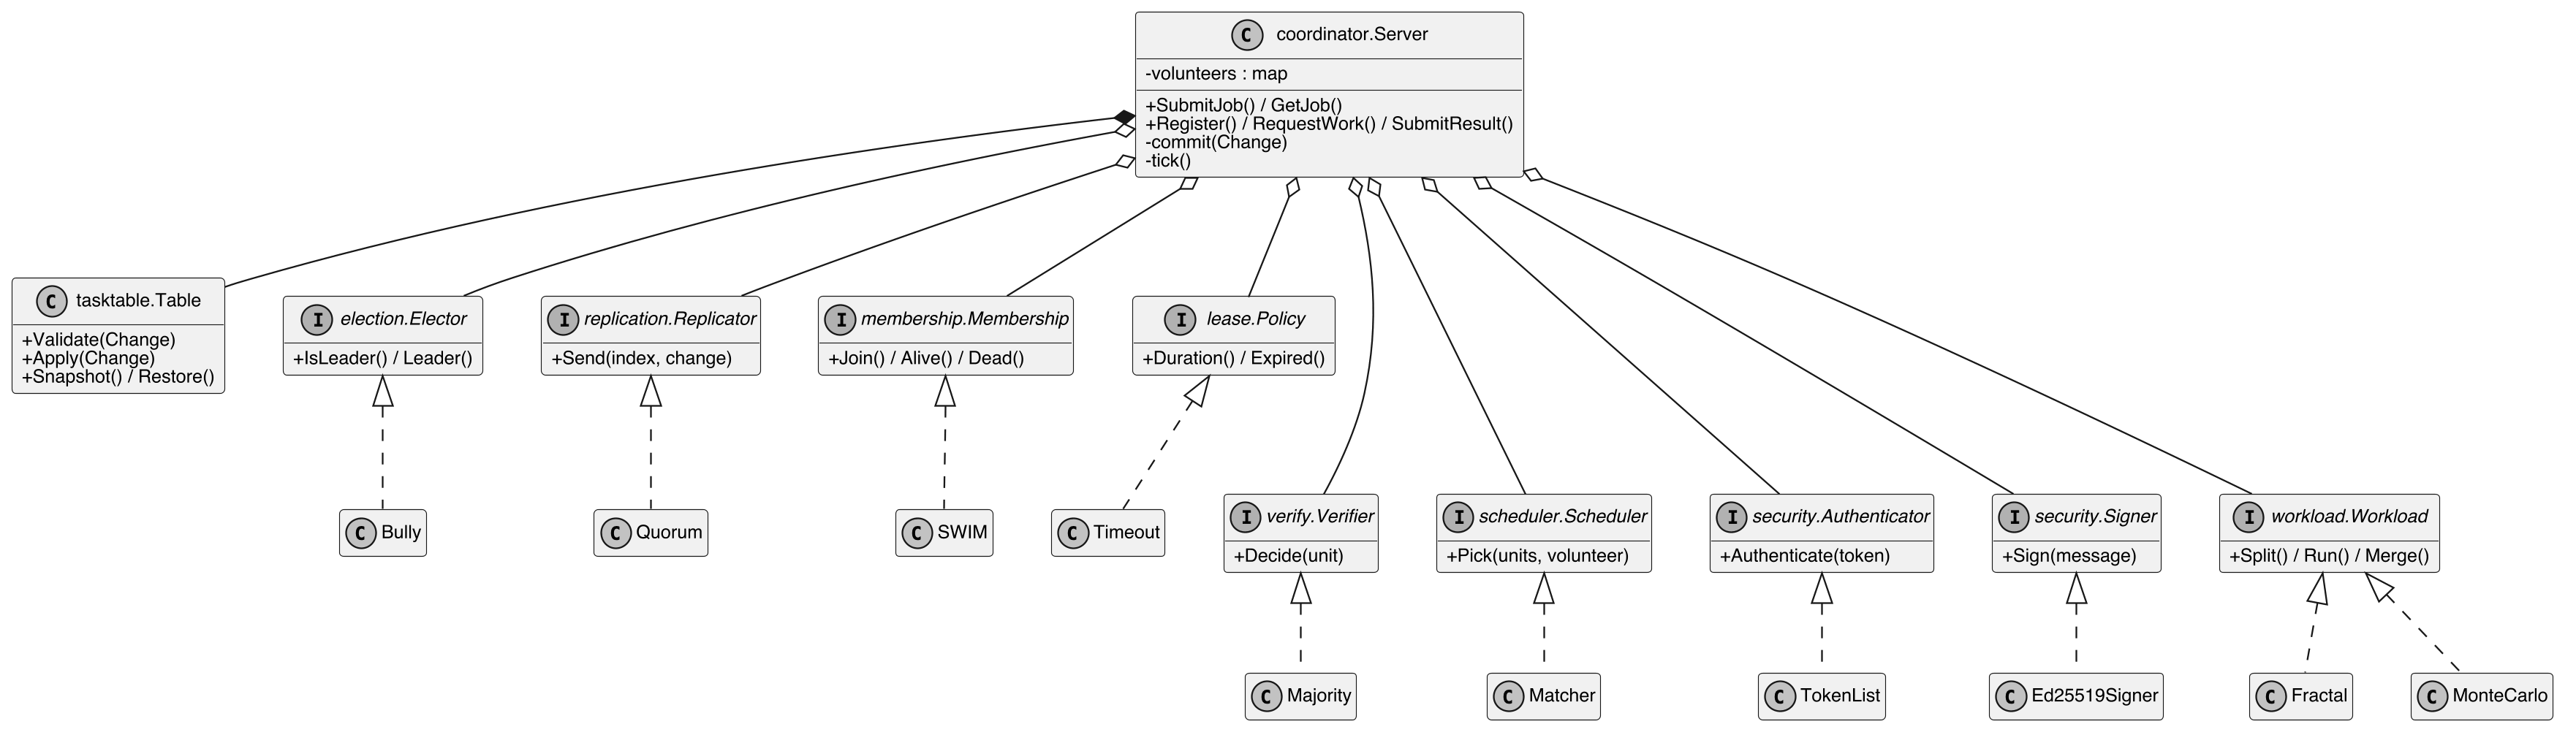
\includegraphics[width=\textwidth]{i1-coordinator-classes.png}
\caption{The coordinator and the interfaces of its parts (implementation diagram I1), with the implementations that the coordinator binary uses. The first stubs remain in each package for tests.}
\label{fig:classes}
\end{figure*}

Two rules keep the replicated state machine correct. Applying a change is deterministic: anything that varies, such as identifiers or lease expiry times, is computed by the leader and stored in the change itself. And every change is validated before it is replicated, under a single mutex that orders all changes, so a backup never receives a change that the leader would then reject.

\todo{Abhishek: implementation diagram I2 (component diagram of the Go packages). Tejas: implementation diagram I3 (object diagram of the task table during a job).}

\subsection{Software Components and Their Interaction}
\label{sec:components}
The system is written in Go and consists of three main programs (coordinator, volunteer and client) and two tools (a key generator and a load generator). All network communication uses gRPC with Protocol Buffers. One contract file defines five services:

\begin{itemize}
\item \texttt{ClientService} (client to leader): submit a job, read its progress and result.
\item \texttt{VolunteerService} (volunteer to leader): register, request work, submit a result.
\item \texttt{ElectionService} (coordinator to coordinator): election, coordinator announcement, heartbeat.
\item \texttt{ReplicationService} (leader to backups): replicate one change, send a snapshot.
\item \texttt{GossipService} (any member to any member): ping and indirect ping.
\end{itemize}

Only the leader serves client and volunteer requests; a follower answers with the gRPC status \texttt{FAILED\_PRECONDITION}. Clients and volunteers hold one connection to every coordinator and send each call to the coordinator that answered last, moving on to the next one when the answer is \texttt{FAILED\_PRECONDITION} or \texttt{UNAVAILABLE}. This one rule makes leader failover transparent to them. Volunteers run their own small gRPC server for gossip only.

Every setting is an environment variable with a default that works on one machine, so the system runs immediately after a clone. Each coordinator exports Prometheus metrics for every main event, such as units accepted, leases released after a death, gossip members by state and registrations rejected. Tests run complete jobs inside one process over in-memory gRPC connections, and the continuous integration pipeline runs every test with the Go race detector on each change.
